\subsection{Liquid Experiments}

We have also tested tritium removal from liquid xenon.  Our liquid xenon system consists of two main sections, the CH$_3$T injection system and the liquid xenon system.  We will first discuss the set up of the tritium injection system, pictured below.

\begin{figure}[h]
\centering
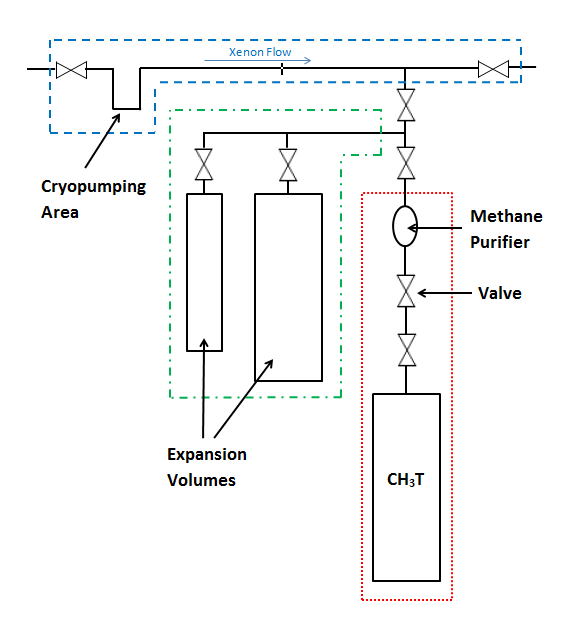
\includegraphics[scale=0.4]{UMDInjectionSys.png}
\caption{The tritium injection system for the liquid phase experiments at UMD. The red box indicates the CH$_3$T storage bottle and methane purifier area, the green box indicated the expansion volumes, and the box indicates the cryopumping and xenon flow through area.}
\label{fig:UMDSys}
\end{figure}

The injection system begins at the CH$_3$T storage bottle.  This bottle is double valved for safety reasons.  As with the gaseous experiments, we have a SAES MC1-905F methane purifier in series with the storage bottle.  Following the methane purifier there is a series of injection volumes branching off to the left.  These injection volumes are designed to inject the desired amount of CH$_3$T into the xenon system.  The last component of the injection system is located above the injection volumes.  This plumbing is used to collect all of the CH$_3$T from the injection volume via cyropumping.  After the plumbing has warmed, the xenon circulating outside of the injection system is rerouted through the cryopump plumbing to sweep all of the CH$_3$T into the xenon system.

The second section of our system, the liquid xenon system, is pictured below.

\begin{figure}[h]
\centering
\includegraphics[scale=0.5]{cryo.png}
\caption{The liquid xenon system at UMD. (A) The xenon condenser consists of a helical coil cooled by a pulse tube refrigerator.  (B) The liquid xenon storage vessel houses two PMTs to observe tritium decay.}
\label{fig:Cryo}
\end{figure}


In the liquid xenon system, a pulse tube refrigerator cools a xenon gas condenser consisting of a helical coil of copper tubing.  The condensed xenon then drips into a liquid xenon storage vessel.  Inside of the liquid xenon storage vessel are two PMTs that face each other. These PMTs are used to observe xenon scintillation light from tritium decay. Once the vessel is filled both of these PMTs are submerged in the liquid xenon.  Note that this means the system at UMD is a single phase detector, rather than a dual phase detector like LUX.  Polyethylene or teflon curtains were installed in the inner cryostat to surround the PMTs during some of our data sets.  These curtains of plastic were used to study outgassing effects in our detector.  It should be noted that in the plumbing leading to the liquid xenon system there is a SAES Zirconium getter (pcf4c3r1) used to purify the tritiated methane out of the system when desired.

During our liquid phase experiments, our experimental procedure consisted of taking an adequate amount of background data, injecting CH$_3$T into the liquid xenon, waiting for the CH$_3$T event rate to plateau, then purifying the CH$_3$T out of the xenon.  During the data sets in which teflon or polyethylene curtains were installed around our PMTs we bypassed our purifier after initally purifying away the CH$_3$T so that outgassing effects could be studied.  Injection activities for our liquid phase experiment ranged from 1487 $\pm$ 35.06 Bq to 12164 $\pm$ 1028.11 Bq.  

A detailed list of our purification efficiency measurements in liquid xenon is included in Table 1.  Note that the rise in background rate during our polyethylene runs is due to a change in PMT gain.  Using the lessons learned from the gaseous xenon experiments we were able to achieve an average purification efficiency of 99.999\% in our liquid experiments, where we define our purification efficiency to be

\begin{center}
Purification Efficiency $= 1 - \frac{A - B}{I - B},$
\end{center}

\noindent
where $A$ is the background event rate after injecting CH$_3$T, $B$ is the background event rate prior to injecting CH$_3$T, and $I$ is the injected CH$_3$T activity as observed by out PMTs.  We find that the addition of plastic curtains around our PMTs does not impair our ability to remove CH$_3$T at $>$ 99.998\% levels.  To illustrate the effectiveness of CH$_3$T removal, an overlay of injected and purified CH$_3$T spectra is included in Figure \ref{fig:SpectraOverlay}.  

\begin{sidewaystable}
\scalebox{0.8}{
\centering
\caption{CH$_3$T purification efficiencies in liquid xenon.}
\begin{tabular}{ c | c | c | c | c }
Observed Injection Activity (Bq) & Background Before Injection (Bq) & Background After Injection (Bq) & Purification Efficiency & Type of Plastic \\
\hline
10415 $\pm$ 140 & 4.78 $\pm$ 0.38 & 4.99 $\pm$ 0.39 & 0.99998 $\pm$ 0.000054 & No Plastic \\
3295 $\pm$ 46 & 4.99 $\pm$ 0.39 & 5.01 $\pm$ 0.39 & 0.99999 $\pm$ 0.00017 & No Plastic \\
2836 $\pm$ 22 & 5.01 $\pm$ 0.39 & 4.76 $\pm$ 0.39 & 1.00009 $\pm$ 0.00020 & No Plastic \\
12164 $\pm$ 1028 & 4.72 $\pm$ 0.39 & 5.09 $\pm$ 0.39 & 0.99997 $\pm$ 0.000082 & No Plastic \\
11033 $\pm$ 1766 & 5.09 $\pm$ 0.39 & 4.69 $\pm$ 0.38 & 1.00004 $\pm$ 0.00015 & No Plastic \\
9435 $\pm$ 180 & 3.74 $\pm$ 0.38 & 5.32 $\pm$ 0.39 & 0.99983 $\pm$ 0.000061 & Stock Teflon \\
7666 $\pm$ 226 & 5.11 $\pm$ 0.39 & 5.23 $\pm$ 0.39 & 0.99998 $\pm$ 0.000082 & Stock Teflon \\
6043 $\pm$ 446 & 5.23 $\pm$ 0.39 & 5.23 $\pm$ 0.39 & 1.00000 $\pm$ 0.00016 & Stock Teflon \\
4504 $\pm$ 220 & 4.64 $\pm$ 0.39 & 4.71 $\pm$ 0.40 & 0.99998 $\pm$ 0.00016 & No Plastic \\
1487 $\pm$ 35 & 5.79 $\pm$ 0.41 & 5.76 $\pm$ 0.41 & 1.00002 $\pm$ 0.00043 & LUX Polyethylene \\
\end{tabular}
}
\end{sidewaystable}

\twocolumn

\begin{figure}[h]
\centering
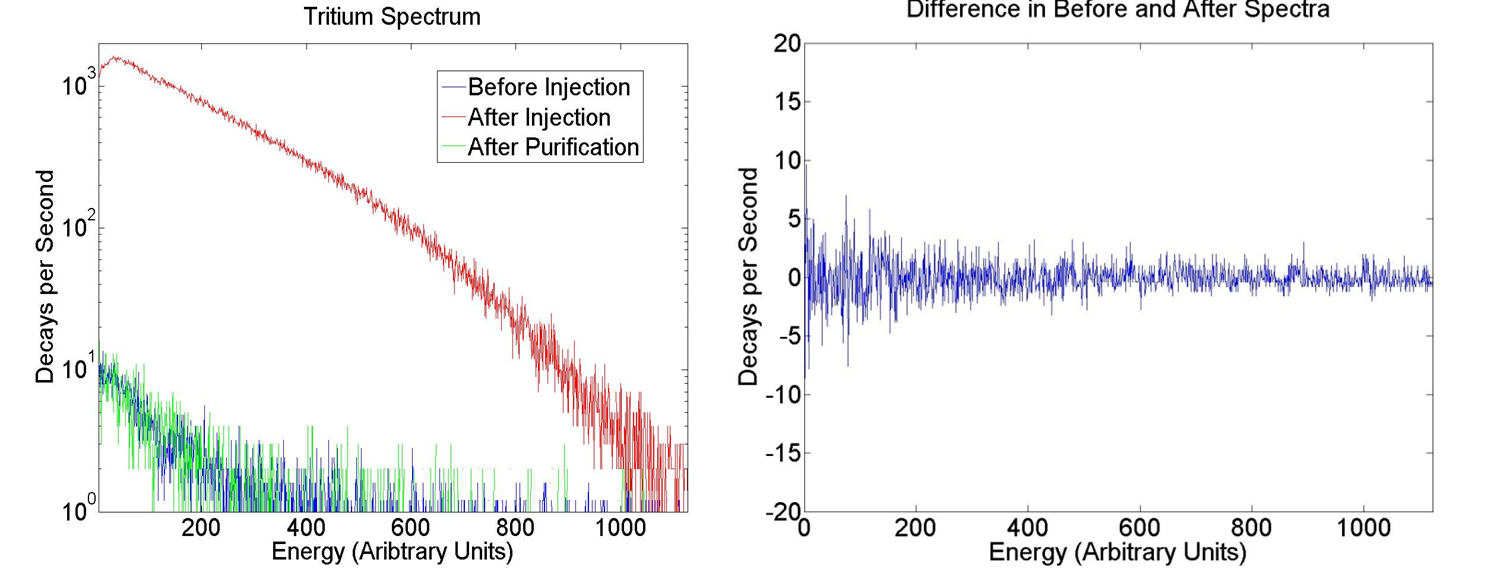
\includegraphics[scale=0.25]{spectra.png}
\caption{Left: Overlay of spectra seen by PMTs in the liquid xenon detector.  The blue spectrum is what is seen by the PMTs prior to injecting tritium, the red spectrum is what is seen by the PMTs after injecting tritium, and the green spectrum is what is seen by the PMTs after purifying the xenon to remove any injected tritiated methane.  Right: The difference between the before injection and after purification spectra.}
\label{fig:SpectraOverlay}
\end{figure}

Cumulatively, we have injected over 68,000 observed becquerel of CH$_3$T into our liquid xenon.  Although systematic errors lead to a fluctuation of our residual background rates, we see no upward trend in our data set as the cumulative observed injection activity rises.


\begin{figure}[h]
\centering
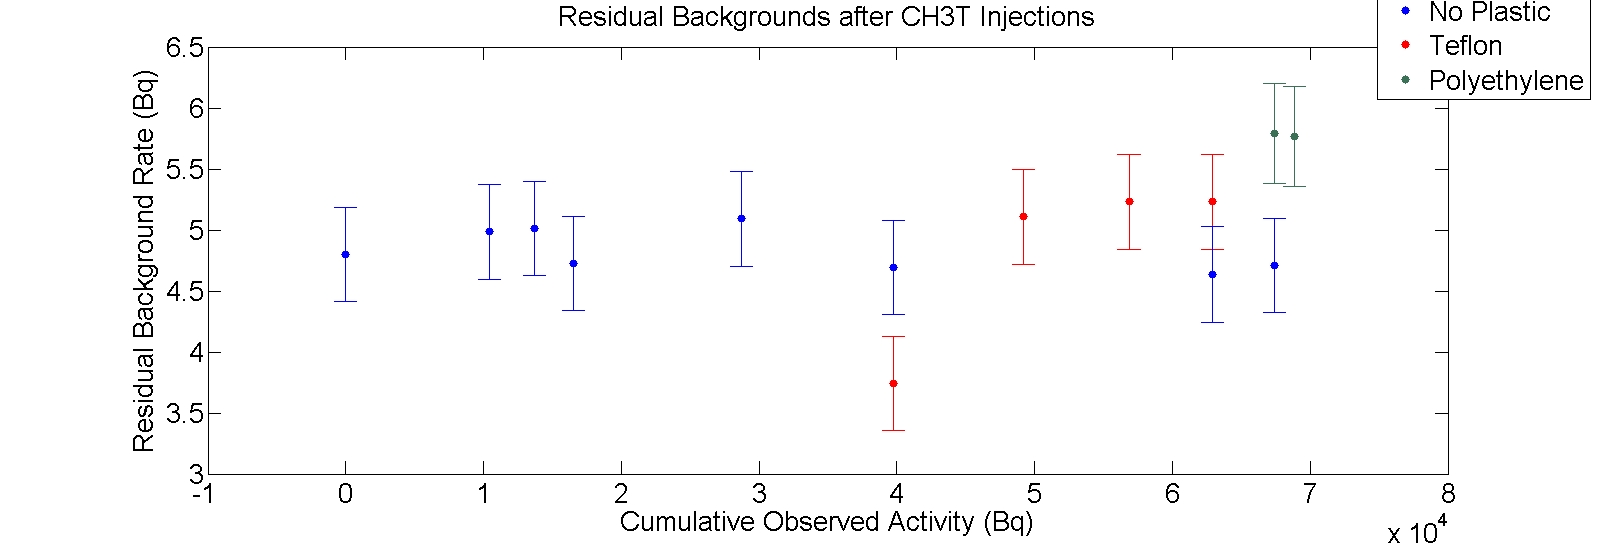
\includegraphics[scale=0.15]{ResidualBackgroundCorrected_SystemErr.png}
\caption{Residual background rates over time in our detector after purifying the CH$_3$T out of the xenon. Blue data points are data sets in which no plastic curtains where used inside of the detector, red data points are data sets in which teflon curtains where used inside of the detector, and green data points are data sets in which polyethylene curtains were used inside of the detector.}
\label{fig:ResBack}
\end{figure}

